\documentclass[aspectratio=169,10pt]{beamer}

% ----------------------------
% Fonts and typography
% ----------------------------
\usepackage{lmodern}
\renewcommand{\familydefault}{\sfdefault} % Computer Modern Sans Serif

% ----------------------------
% Packages
% ----------------------------
\usepackage{amsmath, amsfonts}
\usepackage{graphicx}
\usepackage{booktabs}
\usepackage{tikz}
\usepackage{pgfplots}
\usepackage{enumitem}
\usepackage{tcolorbox}
\usepackage{hyperref}
\pgfplotsset{compat=1.18}

% ----------------------------
% Theme and layout
% ----------------------------
\setbeamertemplate{navigation symbols}{}
\setbeamercolor{frametitle}{fg=blue!70!black}
\setbeamercolor{title}{fg=blue!70!black}
\setbeamerfont{frametitle}{series=\bfseries}
\setlist[itemize]{noitemsep,topsep=2pt,partopsep=0pt,parsep=0pt,leftmargin=*}
\setlength{\abovedisplayskip}{4pt}
\setlength{\belowdisplayskip}{4pt}

% (Header/footer intentionally disabled for clean slides)

% Box for key equations
\newtcolorbox{keyeq}{
  colback=blue!3,
  colframe=blue!50!black,
  boxrule=0.6pt,
  arc=2pt,
  left=6pt,
  right=6pt,
  top=4pt,
  bottom=4pt
}

% Highlighted text box
\newtcolorbox{highlight}{
  colback=yellow!10,
  colframe=yellow!50!black,
  boxrule=0.6pt,
  arc=2pt,
  left=6pt,
  right=6pt,
  top=4pt,
  bottom=4pt
}

% ----------------------------
% Metadata (edit these)
% ----------------------------
\title[Data Science Slides]{Data Science Topic: Template}
\author[Thomaskutty Reji]{Thomaskutty Reji}
\date{}

\begin{document}

% ----------------------------
% Slide 1: Title (optional)
% ----------------------------
\begin{frame}[t]
\titlepage
\end{frame}

% (Table of contents intentionally omitted)

% ----------------------------
% Section 1: Concept Overview
% ----------------------------
\section{Overview}
\begin{frame}[t]{Problem Setup and Motivation}
\begin{columns}[T,onlytextwidth]
\column{0.55\textwidth}
\textbf{Context}
\begin{itemize}
\item One-line problem description.
\item Why it matters for decisions or model quality.
\item Typical pitfalls or failure modes.
\end{itemize}

\textbf{Goal}
\begin{itemize}
\item Short, measurable objective.
\end{itemize}

\column{0.45\textwidth}
\begin{highlight}
\textbf{Key takeaway}\newline
State the main insight in one or two lines.
\end{highlight}
\end{columns}
\end{frame}

% ----------------------------
% Section 2: Equations
% ----------------------------
\section{Core Equations}
\begin{frame}[t]{Main Equation (Boxed)}
\begin{keyeq}
\[
\text{Objective} = \arg\min_{\theta} \; \sum_{i=1}^{N} \ell(y_i, f(x_i;\theta)) + \lambda \Omega(\theta)
\]
\end{keyeq}
\small
Where $\ell$ is the loss, $\Omega$ is the regularizer, and $\lambda$ controls complexity.
\end{frame}

% ----------------------------
% Section 3: Table Example
% ----------------------------
\section{Tables}
\begin{frame}[t]{Example Table}
\begin{table}
\centering
\begin{tabular}{lcc}
\toprule
Method & Metric A & Metric B \\
\midrule
Baseline & 0.72 & 0.31 \\
Improved & 0.81 & 0.25 \\
\bottomrule
\end{tabular}
\end{table}
\end{frame}

% ----------------------------
% Section 4: Figure Example
% ----------------------------
\section{Figures}
\begin{frame}[t]{Figure Placeholder}
\begin{columns}[T,onlytextwidth]
\column{0.6\textwidth}
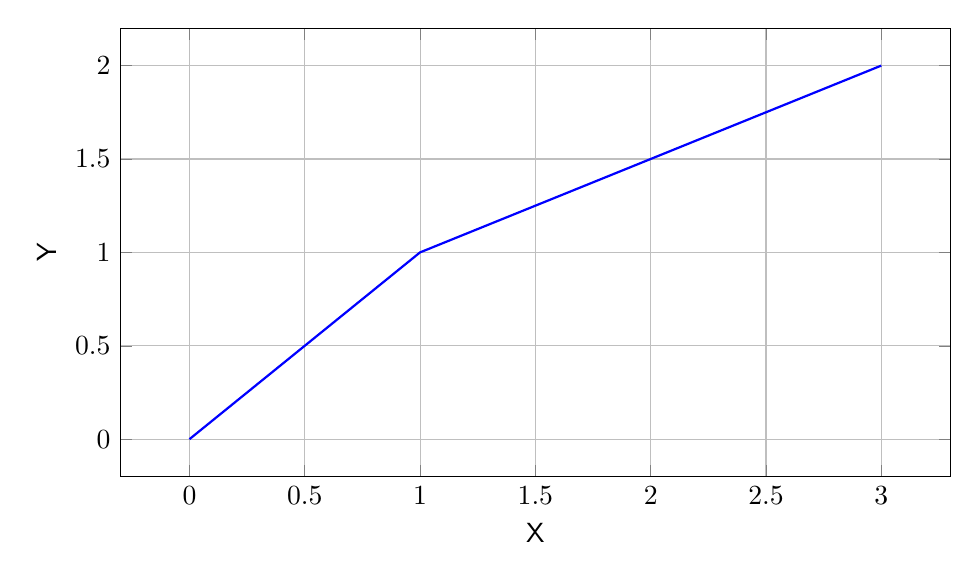
\begin{tikzpicture}
\begin{axis}[
    width=\linewidth,
    height=0.6\linewidth,
    xlabel={X},
    ylabel={Y},
    grid=both,
]
\addplot[thick, blue] coordinates {(0,0) (1,1) (2,1.5) (3,2)};
\end{axis}
\end{tikzpicture}

\column{0.4\textwidth}
\textbf{Notes}
\begin{itemize}
\item Explain what the figure shows.
\item Mention key trend or anomaly.
\end{itemize}
\end{columns}
\end{frame}

% ----------------------------
% Section 5: Summary
% ----------------------------
\section{Summary}
\begin{frame}[t]{Summary}
\begin{itemize}
\item Bullet 1: outcome or result.
\item Bullet 2: recommended action or next step.
\item Bullet 3: caveat or limitation.
\end{itemize}
\end{frame}

\end{document}
